\section{Compatibility with Driver-Ecosystem}
\label{sec:programmingModel}

% CONTENT:
% - System components (AE, CE, PE)
%   - why did we go this way?
% - Isolation within a CE
% - How attestation extends to full platform
% - Platform-awareness (what happens when x is killed)

% \ad{Attestation and platform awareness part is revised. Continue with the motivation}

\Nameenclave{} must include the drivers to interact between the distributed enclaves. While there exist bare-metal drivers, this is not common for all devices. Instead, developers will aim to port existing drivers from the operating systems to \name{} which incurs a cost to manually adapt them to a more minimal bare-metal runtime. As such, we propose to 

As we have seen in the previous section (Section~\ref{sec:approach}), \name enables isolated communication between different components within a \nameenclave over shared memory channels. Hence, we see that \name{}'s hardware architecture is significantly different from traditional operating systems and behaviour of existing applications. Hence, \name poses a significant challenge to the developers to retrofit existing applications to fit within \name{}, violating one of the main design goals of \name to retain similar flexibility and usability to modern operating systems. In this section, we introduce \name{}'s programming model that aims to provide similar flexibility as modern OS's, namely by allowing multiple applications to access the same peripheral simultaneously. The programming model also tries to reduce the effort from developers to adapt existing applications to \name{}'s hardware architecture. This is achieved by providing an abstraction layer over the underlying hardware architecture that hides the lower level complexity. Our programming model dictates how developers can write applications, peripheral drivers, or peripheral firmware and how these entities talk to each other. Moreover, it allows flexible attestation of all its components. Note that the \name{}'s programming model is independent of the \name{}'s hardware architecture (refer to Section~\ref{sec:approach}). For example, if a TEE implements the inter-enclave communication over the file system rather than the shared memory that we propose, or is based on Intel SGX instead, the programming model remains unchanged.

\begin{figure}[t]
\centering
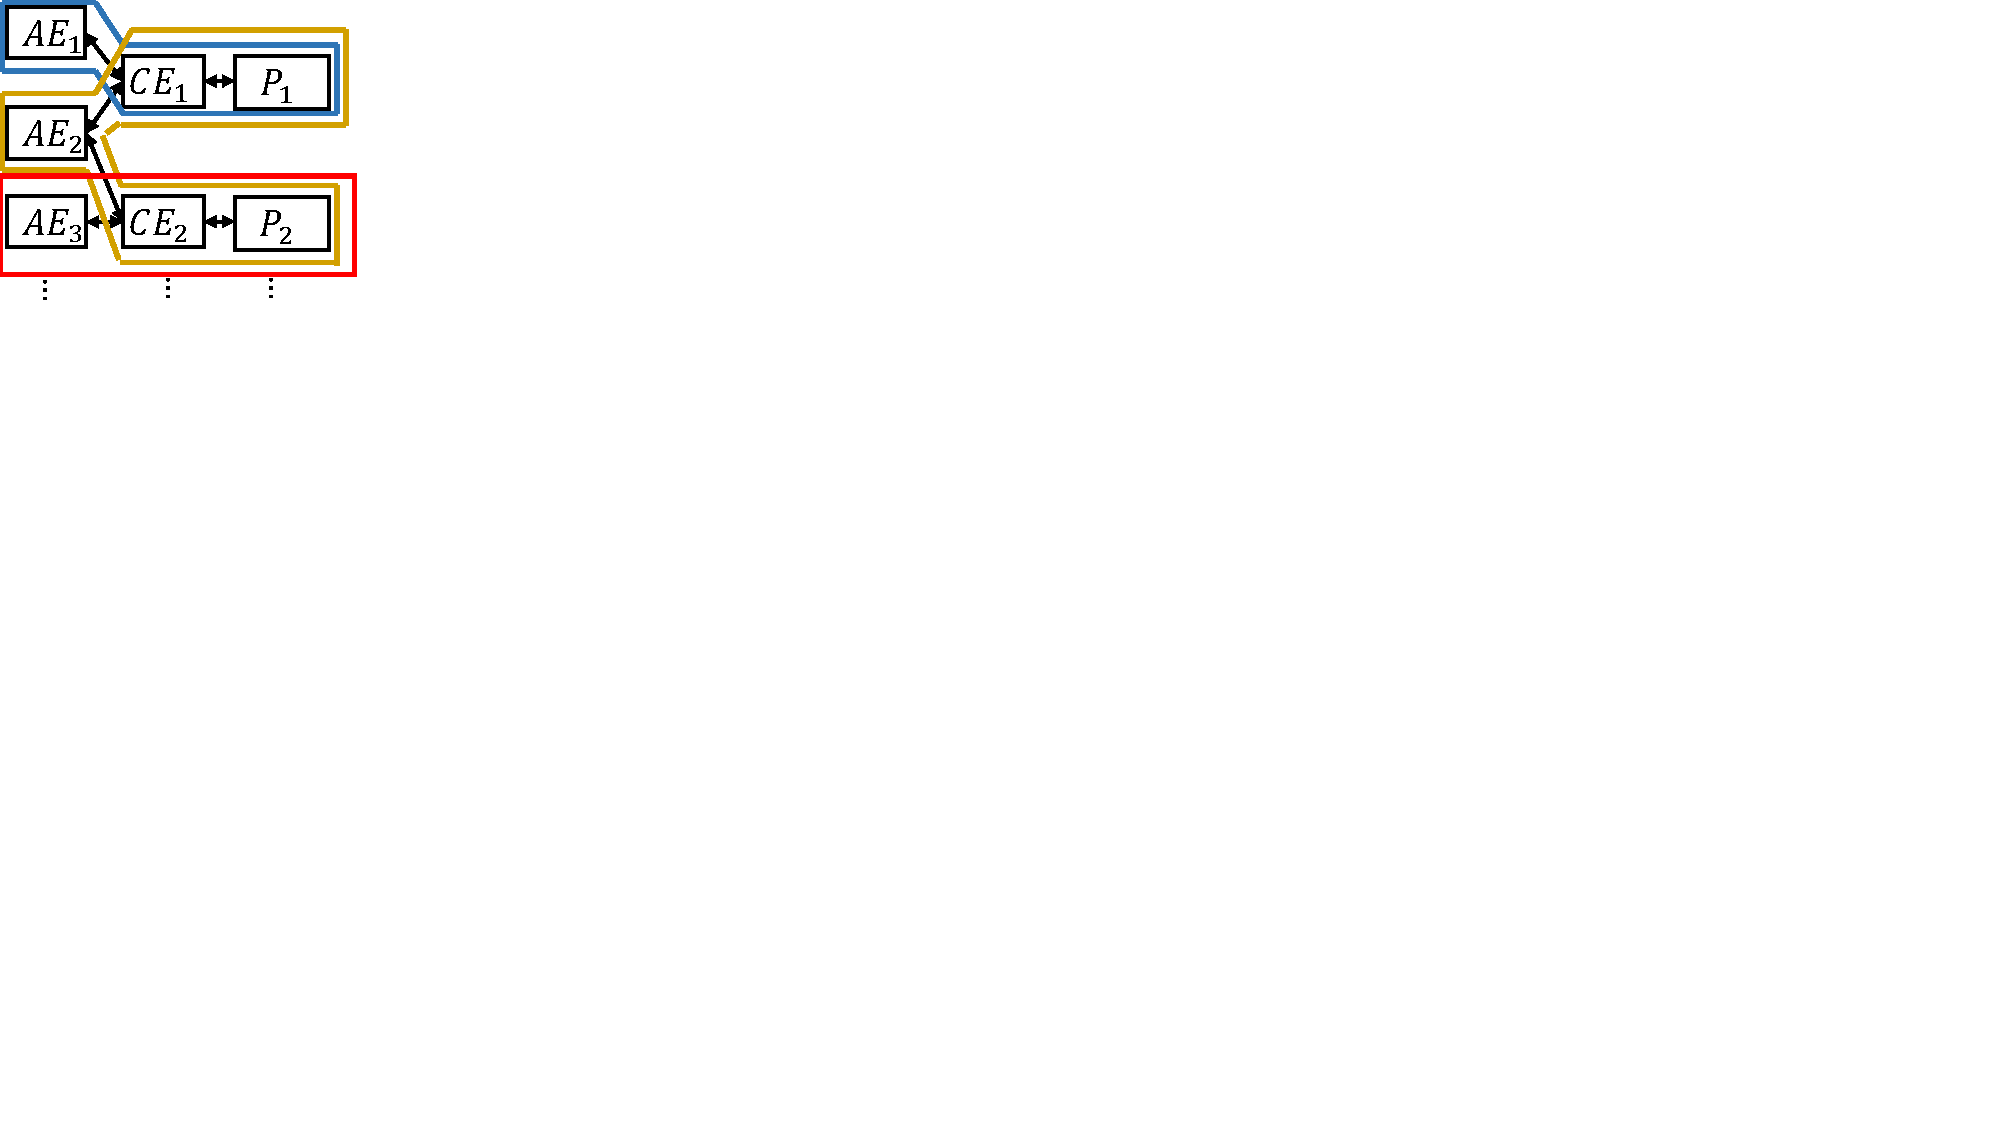
\includegraphics[trim={0 14cm 28cm 0}, clip, width=0.42\linewidth]{programmingModelComponents.pdf}
\caption{\textbf{\name programming model.} The application enclaves (AE) contains the application logic and communicate with peripherals through controller enclaves (CE) that contains the driver logic for the specific peripheral. In our programming model, we assume that there is only one \ce per peripheral. Multiple \app can connect to one \ce{}, and one \app can connect to multiple \ce. Three separate \nameenclave{}s are indicates by the blue, yellow and red outlines.}
\label{fig:programmingModelComponents}
\end{figure}

\subsection{System components}
\label{sec:programmingModel:systemComponents}

\name's programming model consists of three types of entities: \app{}s, \ce{}s, and peripherals as shown in Figure~\ref{fig:programmingModelComponents}. The first two are similar to traditional enclaves that run only on the processor, as seen in Intel SGX or Keystone. Peripherals, on the other hand, are external heterogeneous devices that are attached to the platform. Even though enclaves and peripherals are very distinct entities, in \name's programming model, we abstract them be to be homogeneous isolated execution environments. Hence, to developers, they appear to be instances of the same isolated execution environments, irrespective of whether it is an enclave running on the processor core or an external peripheral. All the enclaves and peripherals utilize shared memory to communicate with each other and use the identical system calls and attestation procedures. Together, they can form a platform-wide enclave that spans over multiple components.


\subsubsection{Application Enclaves} 
\label{sec:programmingModel:systemComponents:ae}

Application enclaves are very similar to the established enclaves in Intel SGX or Keystone. In such a traditional TEE, enclaves cannot access peripherals without using the operating system as a mediator, as the OS handles all the drivers. In \name \app{}s also cannot communicate with a peripheral directly. The \app{}s use shared memory to communicate with a \ce that is a peripheral-specific enclave that encapsulates the driver logic. The rationale of separating the driver from the business logic is two-fold, i) to avoid requiring the developers to ship driver code with their application, and ii) one \ce per peripheral allows multiple \app{}s to communicate with that specific peripheral in parallel. %Note the processor may employ memory encryption to encrypt all shared memory regions to protect against a local physical attacker. However, the developer could also add an additional encryption layer on top in order to make the data accessible only between the application enclave and the peripheral (where the \ce works as the untrusted transport layer between the \app and the peripheral). 


\subsubsection{Controller Enclave} 
\label{sec:programmingModel:systemComponents:ce}

%untructed CE -- discussion -- switching
The \ce contains the driver that enables communication with a peripheral. Note that \app{}s, standard (non-enclave) applications, and the OS cannot access the peripherals directly. The only way to communicate with a peripheral is through the \ce corresponding to said specific peripheral. Such a design choice isolates the peripheral device drivers: one compromised driver does not affect other peripherals. The \ce maintains an isolated communication channel over shared memory (e.g., in RISC-V, the PMP entry corresponding to a shared memory ensures that only participating enclaves have access to that shared memory) to \app{}s and the peripheral. To simplify the configuration, we assume that only one active \ce per peripheral exists at a time. However, any \ce can be replaced at the user's request. %Note that \ce is the only way to access a specific peripheral. All the other non-enclave applications running on the OS need to connect the \ce (in contrast to the standard OS device driver) to access a peripheral.  

\paragraph*{Isolation of multi-\app session} In \name, multiple \app{}s could connect to a single \ce in order to have simultaneous access to a peripheral. In such a scenario, the \ce keeps separate states corresponding to each of the \app{}s. Note that this is primarily a functional and then a security requirement as operations in one \app could affect the state of computation of another \app in case there is no isolation. For some peripherals, the \ce may need to reset the state of the peripheral when it switches to a session with a different \app (temporal separation). However, for peripherals such as GPU that support multiple isolated workloads in parallel, the state does not have to be reset.



\subsubsection{Peripheral} 
\label{sec:programmingModel:systemComponents:peripheral}

We consider on-chip peripherals as well as external peripherals that are attached to the platform. However, we require them to store some key material from the manufacturer securely for attestation. Similar to \app{}s, peripherals also share memory regions with the \ce that is used as a communication channel. The firmware that runs on peripherals is also part of the platform-wide enclaves. For simple peripherals such as IO devices (keyboard, mouse, etc.), GPS, and temperature sensors, the modification in the firmware is minimal. Essentially, this only includes adding a certificate from the manufacturer that proves that the peripheral is running the correct version of the firmware. %However, for complex peripherals such as GPUs, the developers may require to change the firmware as the GPU needs to isolate the data from multiple \app{}s that execute operations on the GPU simultaneously.

\begin{figure}[t]
  \centering
  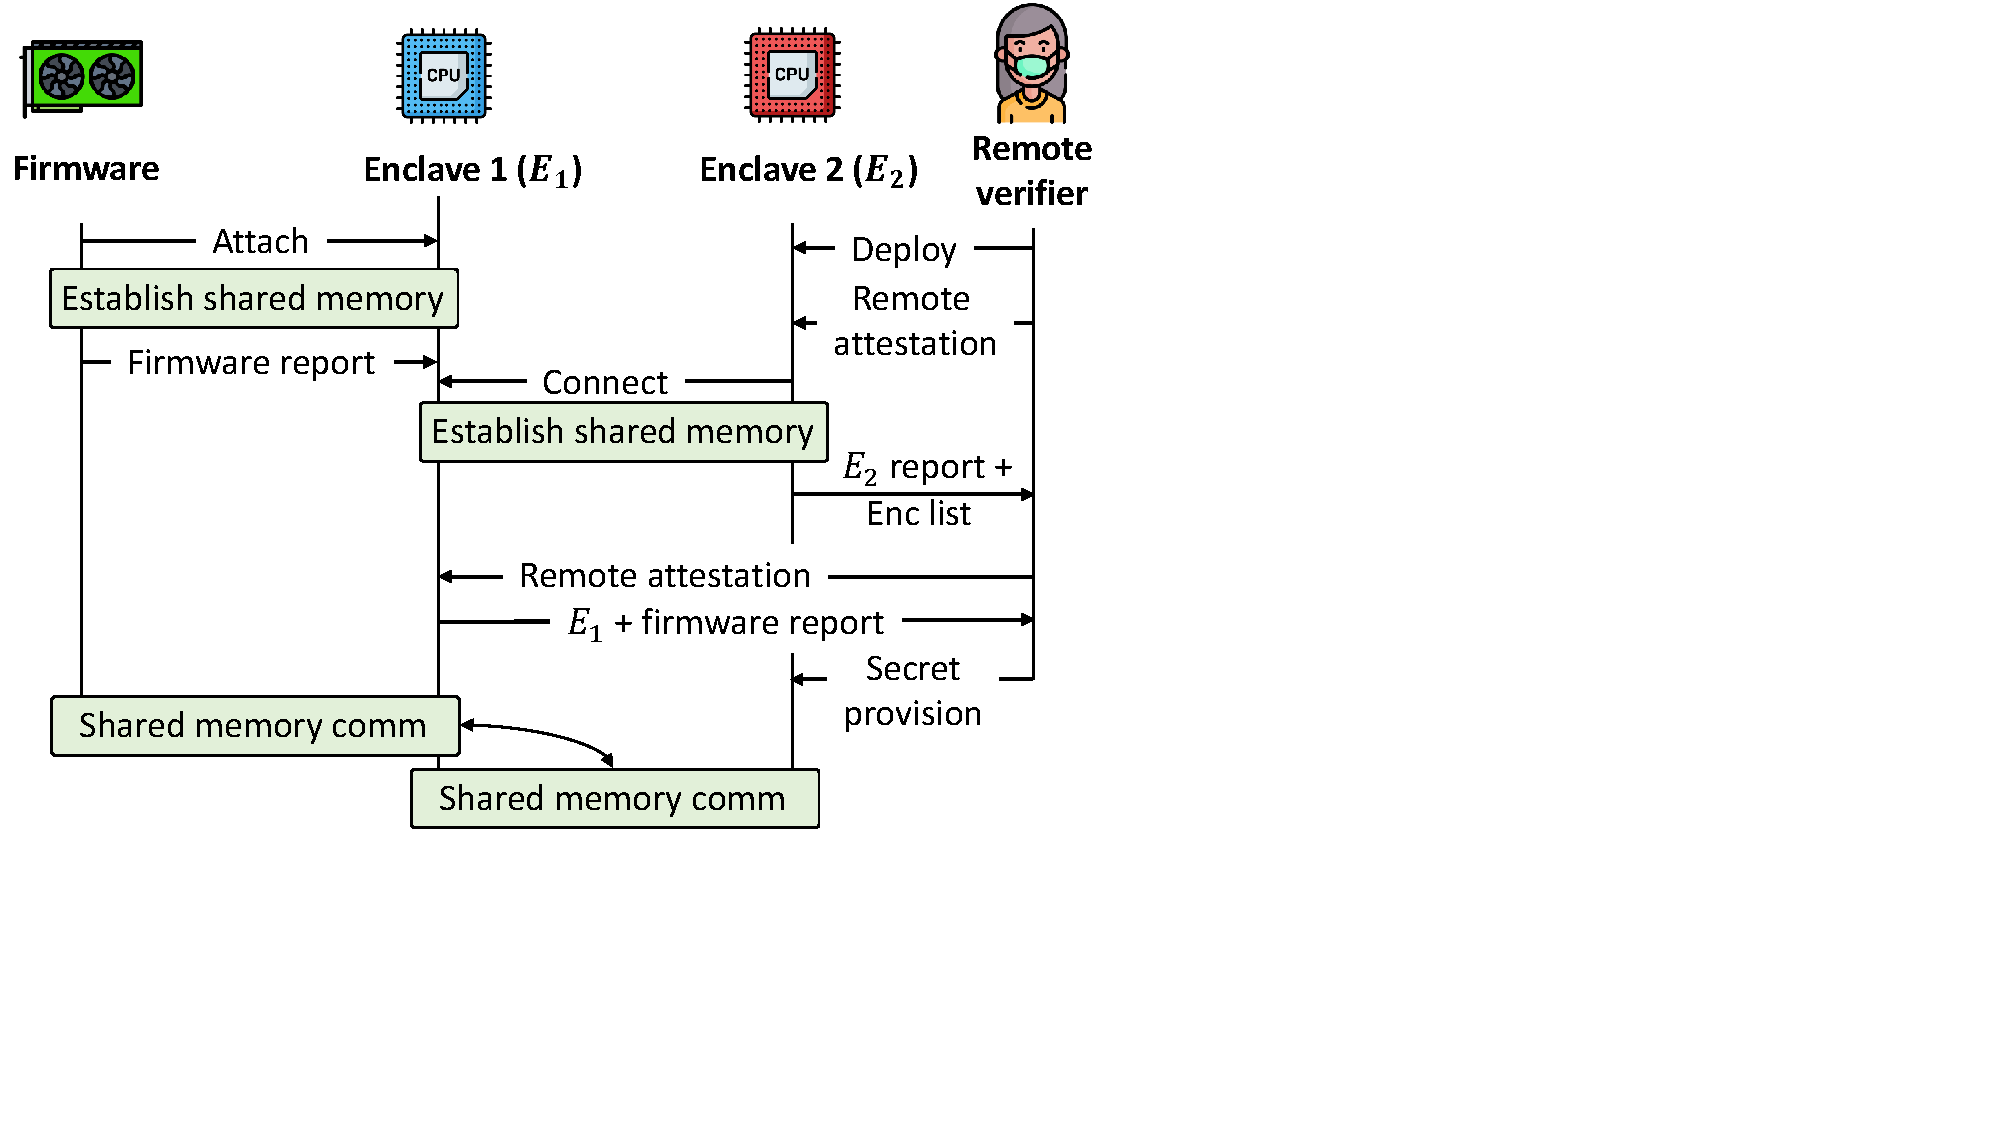
\includegraphics[trim={0 4cm 15cm 0}, clip, width=\linewidth]{localAttestation.pdf}
  \caption{\textbf{Flow of the remote attestation process} between the user, \ce, \app and the firmware.} \vspace{-1.5em}
  \label{fig:attestationFlow}
\end{figure}

\subsection{Platform-wide Attestation}
\label{sec:programmingModel:attestation}

In Section~\ref{sec:approach:attestation}, we provide the hardware construct for \name{}'s platform-wide attestation. In this section, we describe how it related to the programming model components. The platform-wide attestation that enables a remote verifier to verify the state of the \nameenclave components - \app{}s, \ce{}s, and peripherals. Precisely, the state includes the state of the components of the programming model components and their communication channel (over shared memory in our case). Note that there could be more than one verifier (an example is depicted in Figure~\ref{fig:new_system} with two remote verifiers and two \nameenclave{}s) corresponding to several \nameenclave{}s on the same platform. For each remote verifier, the TCB is constrained to only the specific \nameenclave that she is verifying. Hence a remote verifier does not need to trust any \app, \ce or peripheral that she is not using/attesting. Note that platform-wide attestation is built on top of the attestation scheme of the underlying TEE, e.g., the attestation in RISC-V Keystone or Intel SGX. %Enabling  platform-wide attestation requires some modifications of the existing remote attestation procedure of traditional TEEs. 

\subsubsection{Attestation Components}
\label{sec:programmingModel:attestation:components}

The standard attestation report of a traditional enclave contains the following: the measurement of the enclave and the measurement of the low-level firmware (for example, the security monitor in RISC-V keystone). Both of them are signed by the platform key (known as the device root key). For platform-wide attestation, the verifier wants to acquire a signed measurement of the entire \nameenclave{}. That is a combination of signed attestation reports, including the report of the \ce, the configuration of the \ae (initialization parameters), and the signed firmware report of the connected peripherals. We assume that the remote verifier already knows the public keys of the platform and the peripherals.

\paragraph*{Enclave identifiers} When a new processor-local enclave is spawned, the SM assigns a unique identifier to that. This identifier uniquely determines the enclaves participating in a specific shared memory region. When the enclave is killed, the identifier is relinquished.


\subsubsection{Attestation Process between Programming Model Components}
\label{sec:programmingModel:attestation:process}

Figure~\ref{fig:attestationFlow} depicts the sequence of the attestations between different components of the programming model. Note that the platform-wide attestation process starts from the verifier who initiates a remote attestation request of the \app. That, in turn, provide the verifier with the list for connected \ce and subsequently connected peripherals. The sequence of the end-to-end platform-wide attestation is the following:

  
\paragraph{Remote attestation of the \app} The platform-wide attestation process starts with the verifier who wants to attest the deployed \app. The purpose of the remote attestation of the \app is to ensure that the platform is running the intended version of the \app. The \app attestation report includes the list of identifiers of the \ce{}s that have shared memory channels with that \app. This report is signed by the platform's private key. 

\paragraph{Remote attestation of the connected \ce{}s} As mentioned above, the user receives a list of identifiers of \ce{}s that have shared memory channel with the \app. The user then executes a series of individual remote attestation for the \ce{}s. The \ce{}s send the attestation report of themselves along with the certificate that is received from the connected peripherals. These reports are signed by the same platform key as of the \app attestation report. This proves that the \app and the connected \ce{}s are running on the same physical platform. Additionally, the \ce also states that the initiating \app has a shared memory channel with it. At the end of this process, the verifier who initiated the remote attestation of the \app receives the signed attestation report of the said \app, all the \ce{}s that are connected with the \app and all the peripherals that are governed by the \ce{}s.

\paragraph{Local attestation between \ce and peripheral} The local attestation process between a peripheral and a \ce takes place when a new peripheral is attached to the platform. This step is independent of the above mentioned two steps that only starts when the verifier wants to attest a specific \app. When a new peripheral is attached to the platform, \ce gets the list of attached peripherals from the SM (through the device tree). The peripherals come with a certificate that states the firmware version certified by the manufacturer along with the signing key from the manufacturer. The \ce issues a random challenge to the peripheral. It verifies if the peripheral actually owns the private key corresponding to the certificate. The peripheral signs the challenge and sends it back to the \ce for verification.
After the local attestation between the \ce and the peripheral, the \ce knows that is it connected with a legitimate peripheral with a certified firmware.
%, and ii) both the \ce and the peripheral are running on the same platform.
 


\subsection{Platform Awareness}
\label{sec:programmingModel:platformAwareness}

As described in the previous sections, platform-awareness is one of the most important features of \Nameenclave, i.e., the individual enclaves know about the states of other enclaves that are connected to them. Note that it is infeasible that the enclaves keep track of all possible states of other enclaves. In our implementation of \name, we handle specific states such as enclave termination, re-deployment, peripheral attachment, and detachment. Depending on the \app ($AE$), or the \ce ($CE$) or the peripheral, the policy on how to handle the changes in these states in other enclaves are as the following. The specific implementation of how the different components of \Nameenclave know about each other's states is dependent on the underlying hardware architecture. For example, for our implementation of \name, we use the asynchronous disconnect to convey this information, as described in Section~\ref{sec:approach:sharedMemory}. For generality, in this section, we assume that the SM \emph{notifies} the programming model components about each other's state. We denote a shared memory space as $S_{\{E_1, E_2\}}$ when it is shared between two enclaves $E_1$ and $E_2$.


\subsubsection{$AE$ is killed:} Assume that $AE$ communicated with $CE$ over $S_{\{AE, CE\}}$. In such a situation, only the specific shared memory space $S_{\{AE, CE\}}$ is destroyed. At the same time, the SM notifies the $CE$ about the destruction of $AE$. A specific application may require that the peripheral is notified in the case the peripheral is handling sensitive data from $AE$. In such a scenario, the $CE$ tells the specific peripheral that the $AE$ was communicating with to report that the $AE$ is terminated. Note that how the peripheral handles this call is also dependent on the implementation of that peripheral firmware enclave. For example, a peripheral that handles sensitive user data may decide to terminate the session completely (by zeroing out all the internal states) and destroy the shared memory between the peripheral and $CE$. Note that, along with the $AE$, multiple other \app{}s could be connected with the $CE$. In that case, the rest of the communication channels between the other \app{}s and the $CE$ remain intact due to the isolation of shared memory regions enforced by the \ce.
    
\subsubsection{$CE$ is killed:} All the shared memory regions that are associated with the $CE$ (this includes the shared memory spaces with both \app{}s and peripherals) are also zeroed out, and the respective $AE$s are notified by the SM. Zeroing out the shared memory also notify the peripheral that the respective $CE$ is killed. Forcing the peripheral to reset. When the $CE$ is reinitialized, the $CE$ needs to reestablish the communication to the peripheral -- requires the local attestation between the propel and the $CE$ (refer to Section~\ref{sec:programmingModel:attestation:process}). The user of the $AE$ that wants to connect with the $CE$ also needs to perform a remote attestation of the $CE$ to re-verify i) the $CE$ is a legitimate one, and ii) the peripheral that is accessed by the $CE$ is a legitimate one and the shared memory between them is set up as intended.
    
\subsubsection{Peripheral is reattached, or the firmware enclave is changed:} The SM notifies the $CE_p$ about the peripheral ($p$) changes and invalidates $S_{\{p, CE_p\}}$, the shared memory space between the $CE$ and the peripheral. This also results in the destruction of all the shared memory that is associated with $CE_p$ and $p$. All application enclaves $AE$ that use $CE_p$ must be notified. Similar steps are taken if the peripheral is reattached to the platform.

